% \section*{Custom Component}

% \begin{minted}[
%     frame=single,
%     breakanywhere,
%     breaklines
% ]{python}
% from haystack import component, Document
% from typing import List
% import asyncio

% @component
% class DocumentSummarizer:
%     """
%     A component generating summaries for each given document
%     """
%     prompt = """You are a helpful assistant, that summarizes documents very concisely.\n\nSummarize the following document:\n{document}\n\nSummary:"""

%     async def summarize(self, doc: Document):
%         # Summarizing Code

%     @component.output_types(documents=List[Document])
%     def run(self, documents: List[Document]):
%         """Run the component in parallel for multiple documents"""
%         async def async_run():
%             tasks = [self.summarize(doc) for doc in documents]
%             results = await asyncio.gather(*tasks)
%             return {"documents": results}
%         return asyncio.run(async_run())


% \end{minted}


% \newpage

\chapter{Pipeline Diagrams}

\begin{figure}[h]
  \centering
  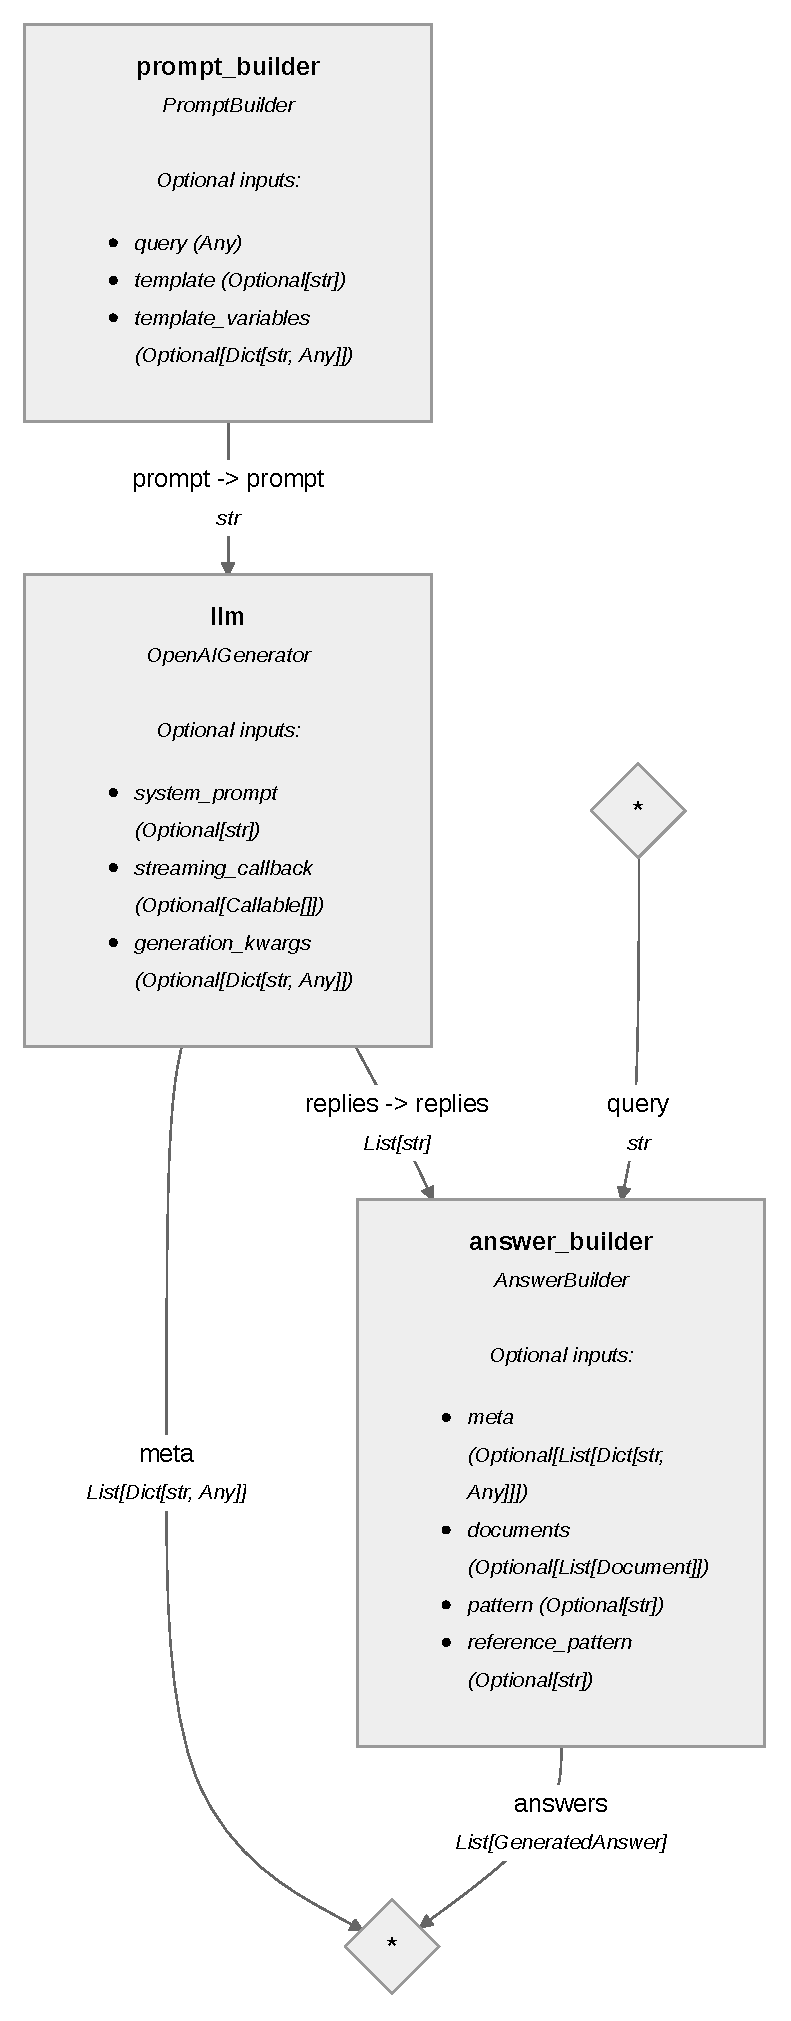
\includegraphics[width=0.35\textwidth]{images/baseline_llm.pdf}
  \caption{Pipeline diagram of the standalone LLM baseline implementation}
  \label{fig:pipeline_llm}
\end{figure}

\newpage

\begin{figure}[h]
    \centering
    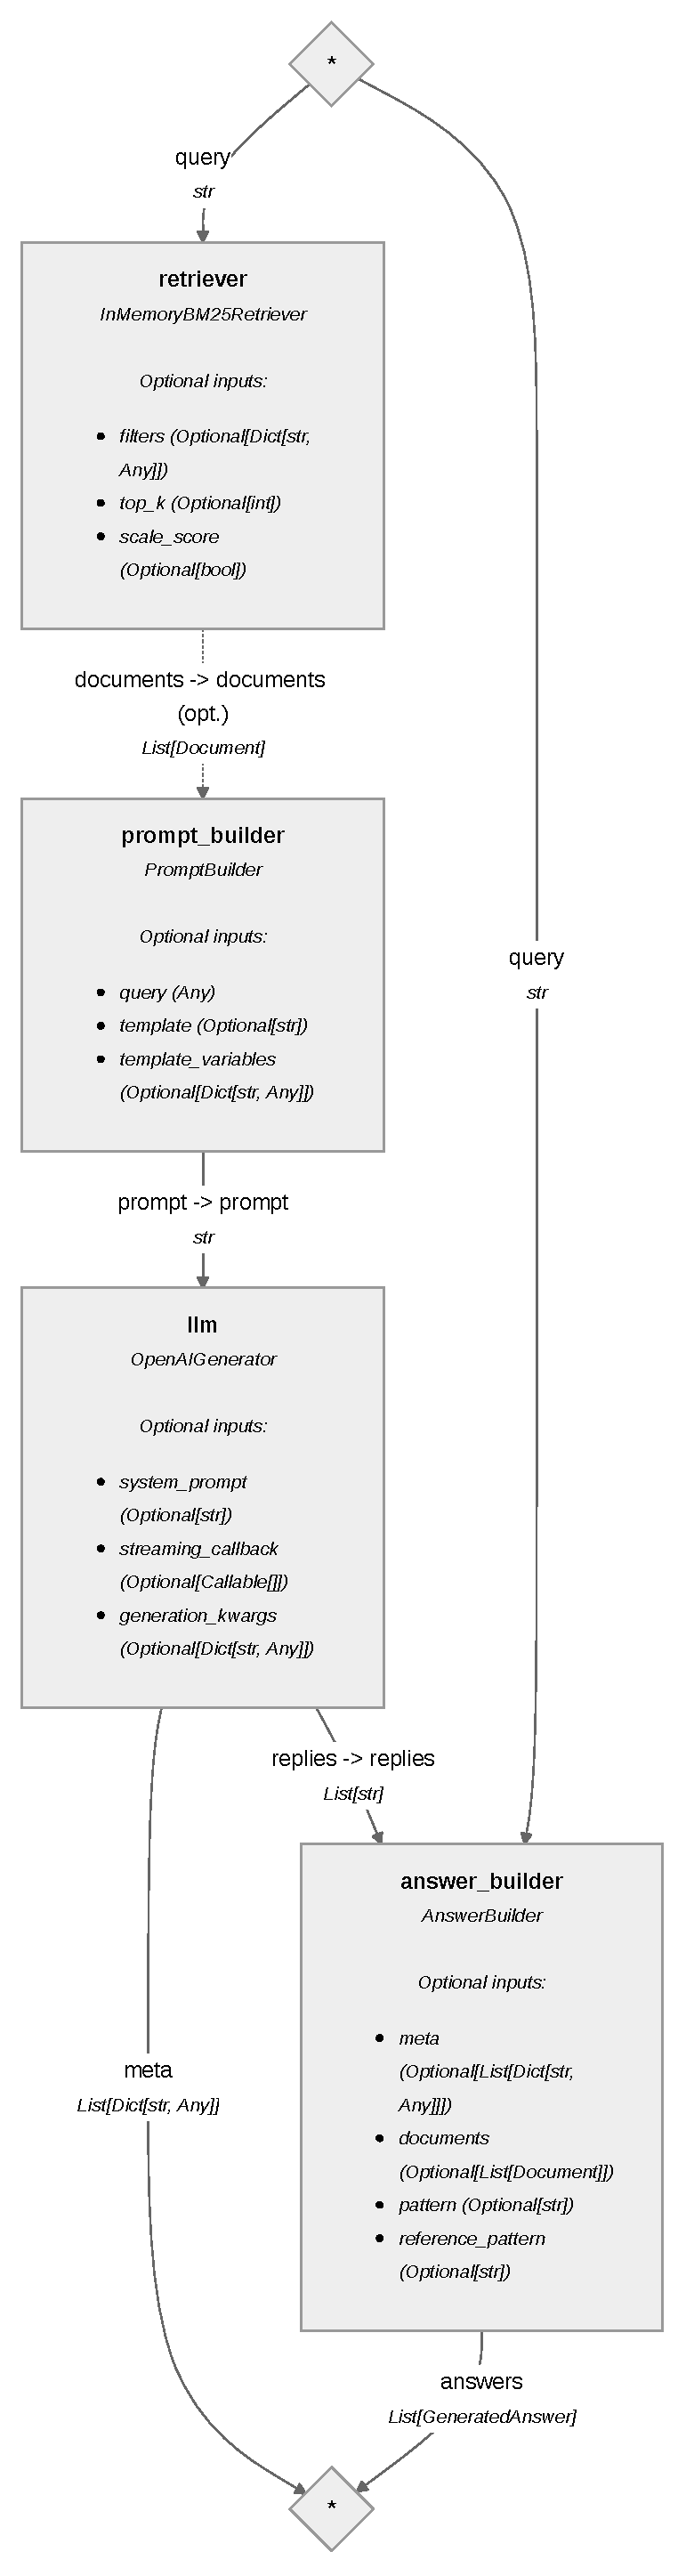
\includegraphics[width=0.37\textwidth]{images/baseline_bm25.pdf}
    \caption{Pipeline diagram of the BM25 baseline implementation}
    \label{fig:pipeline_bm25}
\end{figure}


\newpage

\begin{figure}[h]
    \centering
    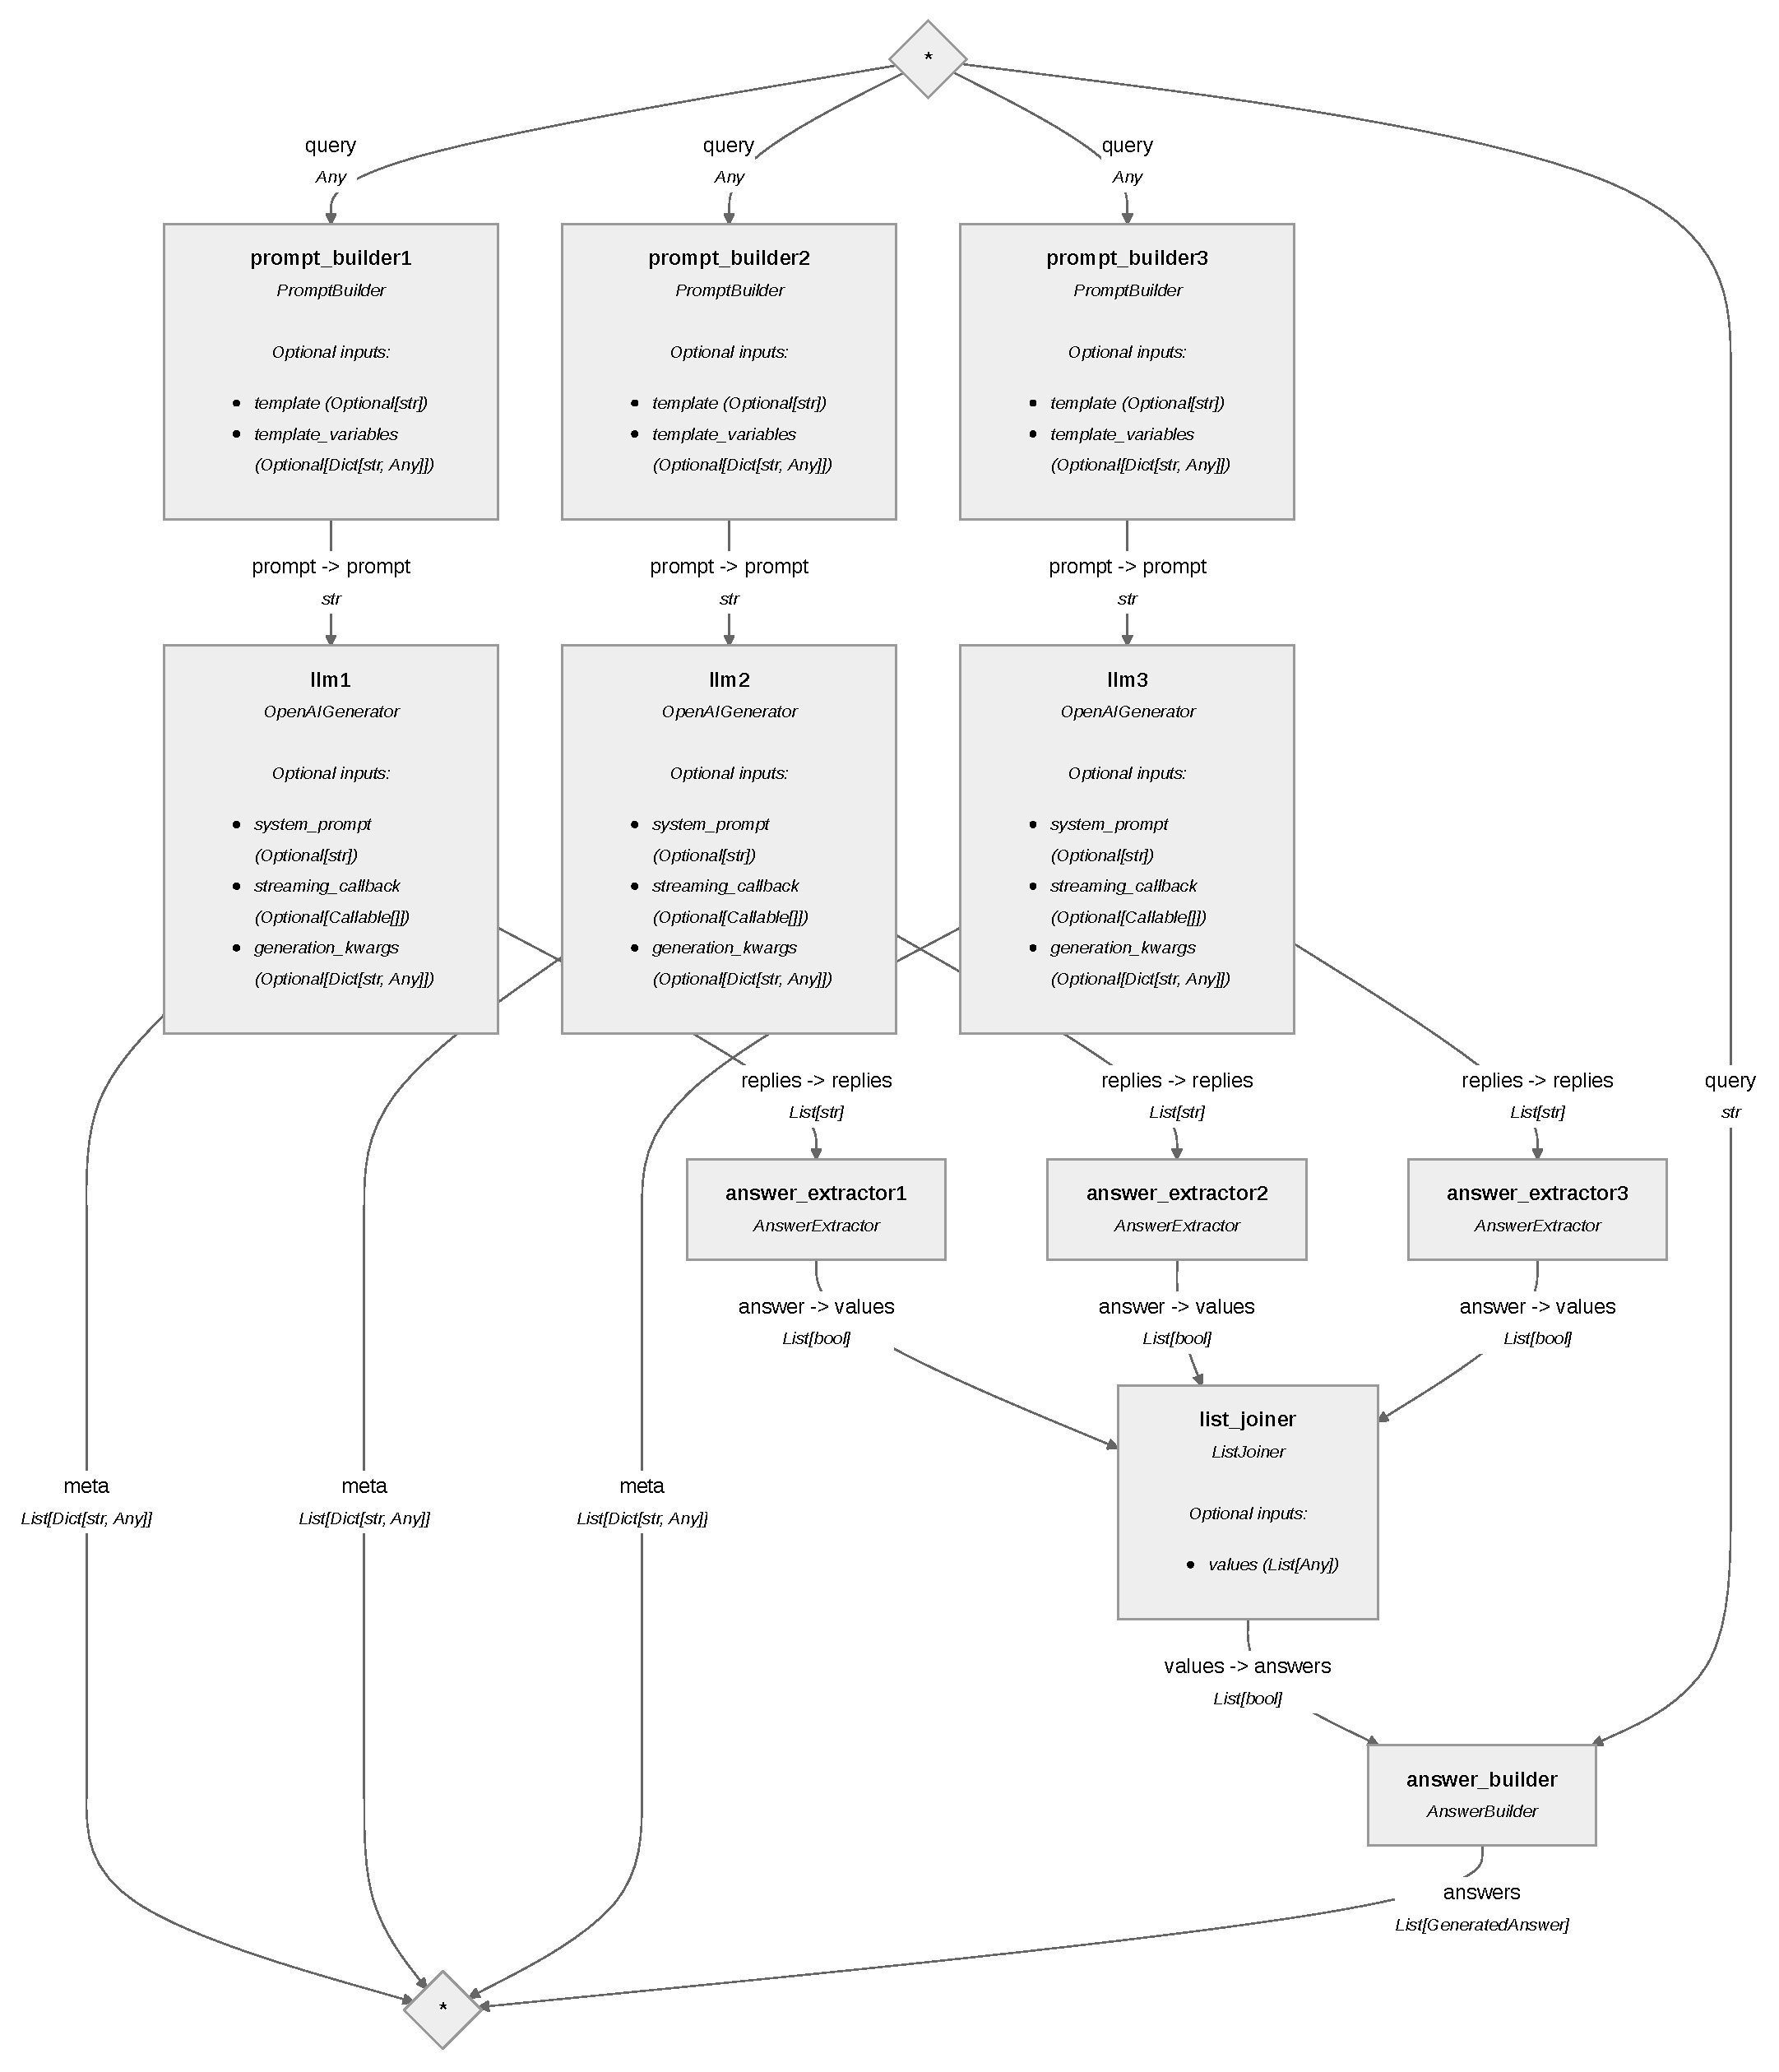
\includegraphics[width=0.95\textwidth]{images/baseline_ciri.pdf}
    \caption{Pipeline diagram of the Ciri baseline implementation}
    \label{fig:pipeline_ciri}
\end{figure}






